
\documentclass[10pt,conference, twocolumn]{IEEEtran}
\hyphenation{op-tical net-works semi-conduc-tor}

\usepackage[utf8]{inputenc}
\usepackage{listings}
\usepackage{color}
\usepackage{kpfonts,dsfont}
\usepackage{graphicx}
\usepackage{float}
\usepackage{algorithm}
\usepackage[noend]{algpseudocode}
\usepackage{amsmath, amsthm, amssymb, amsfonts}
\usepackage{datetime}
\usepackage{listings}
\usepackage{color}
\definecolor{codegreen}{rgb}{0,0.6,0}
\definecolor{codegray}{rgb}{0.5,0.5,0.5}
\definecolor{codepurple}{rgb}{0.58,0,0.82}
\definecolor{backcolour}{rgb}{0.95,0.95,0.92}
\lstdefinestyle{mystyle}{
    backgroundcolor=\color{backcolour},
    commentstyle=\color{codegreen},
    keywordstyle=\color{magenta},
    numberstyle=\tiny\color{codegray},
    stringstyle=\color{codepurple},
    basicstyle=\footnotesize,
    breakatwhitespace=false,
    breaklines=true,
    captionpos=b,
    keepspaces=true,
    numbers=left,
    numbersep=5pt,
    showspaces=false,
    showstringspaces=false,
    showtabs=false,
    tabsize=2
}
\lstset{style=mystyle}


\begin{document}
\title{LangUI: Vector Drawing for Scientific Writing}
\author{Jipeng~Wu}
\markboth{CATEGORY, \currenttime, \today}%
{Shell \MakeLowercase{\textit{et al.}}: Using IEEEtran.cls Template!}
\maketitle


\section{Motivation}
Illustrations in research papers can be classified into 2 categories: data-based charts and concept-based illustrations. We don't usually worry about the first one since data-based charts can be generated automatically. The second one howerver could be painful. Those illustrations may not look like existing graphs or figures that diagramming tools already predefined. They usually try to use basic shapes and lines to convey the concept of a novel model. Existing tools like visio, Lucidcharts, metapost, LaTeXDraw or python support such creation.

But sometimes men are too lazy to drag components or write python/R/TikZ/metapost code.

I want to simply draw what it is in my mind and the software should understand my sketches, tidy up everything and produce some beautiful illustrations.

\section{Objectives}
The highest level goal is to develop a tool that understands users' handdrawing and produce illustrations for scientific writing.

More specifically, it should outperform visio, Lucidchart or code-based tools in efficiency and satisfaction. In terms of completeness and effectiveness, I would not expect full coverage of all features and functions that diagramming tools generally have. However, the LangUI program should at least be able to produce the following illustrations: "lines and curves", "arrows and texts", "basic shapes", "overlapping shapes".

\begin{figure}[H]
\caption{lines and curves}
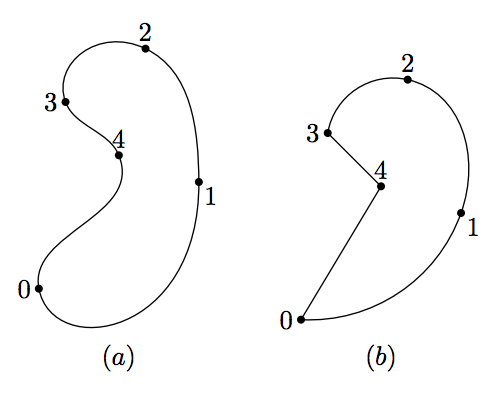
\includegraphics[width=8cm]{1.png}
\end{figure}

\begin{figure}[H]
\caption{arrows and texts}
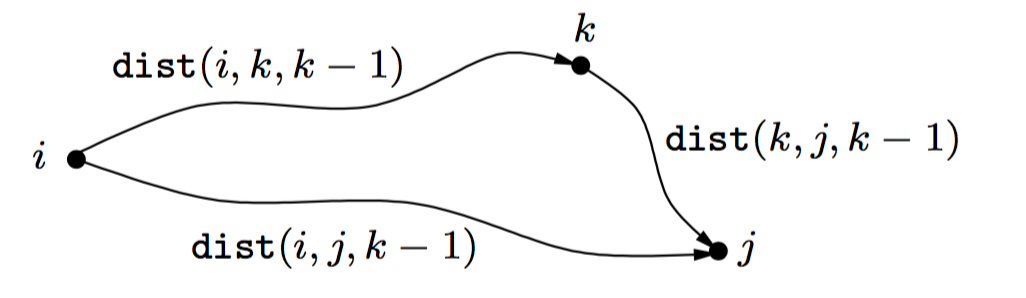
\includegraphics[width=8cm]{2.png}
\end{figure}

\begin{figure}[H]
\caption{basic shapes}
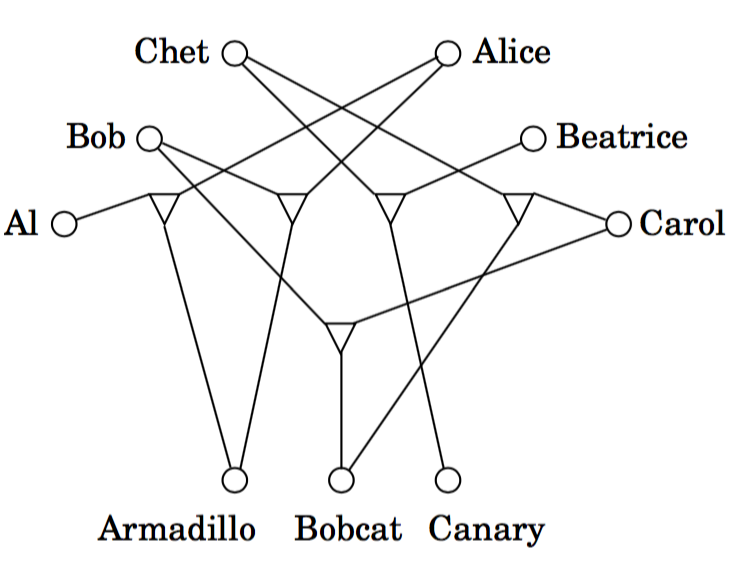
\includegraphics[width=8cm]{3.png}
\end{figure}

\begin{figure}[H]
\caption{overlapping shapes}
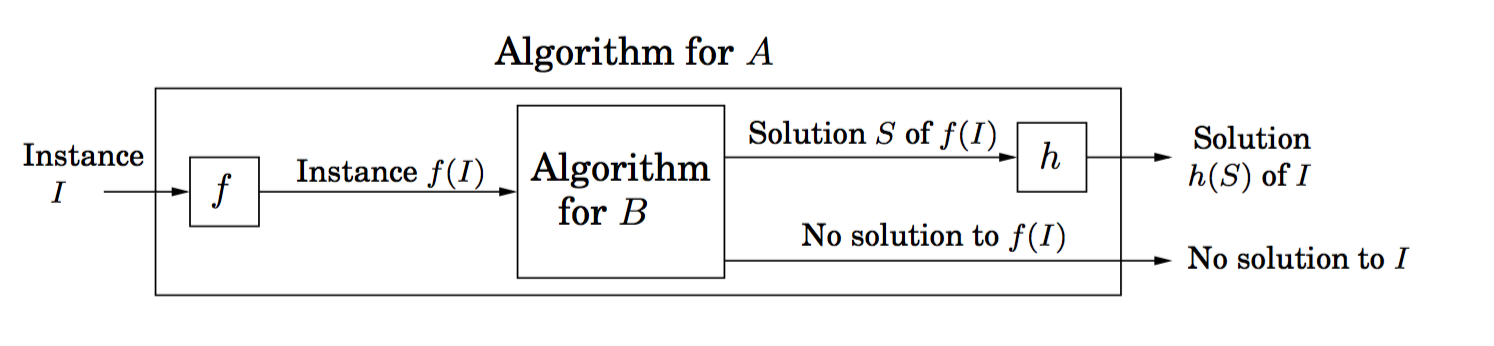
\includegraphics[width=8cm]{4.png}
\end{figure}

Details of measurement of efficiency, satisfaction, completeness and effectiveness will be elaborated later in evaluation phase.

\section{Related work}
Existing digramming tools like visio, Lucidcharts provide a wide range of predefined components. Users select an item and then drag it to some place. When they finish drawing one item, the following item is usually different. So they have to search and click another item. This process is very tiring and especially frustrating when you forget to change the selected item.

Selecting and dragging mode will be a submode in Langui. I think it is still necessary to support this mode. So users are allowed to tweak their layouts after drawing the sketches.

I always want to find a tool that tidy things up and magically makes it look professsional. I haven't found anything like that. But I do find similar ideas exploited in gesture understanding and Chinese stroke input method.


\section{Proposed work}
\begin{figure}[H]
\caption{Architecture}
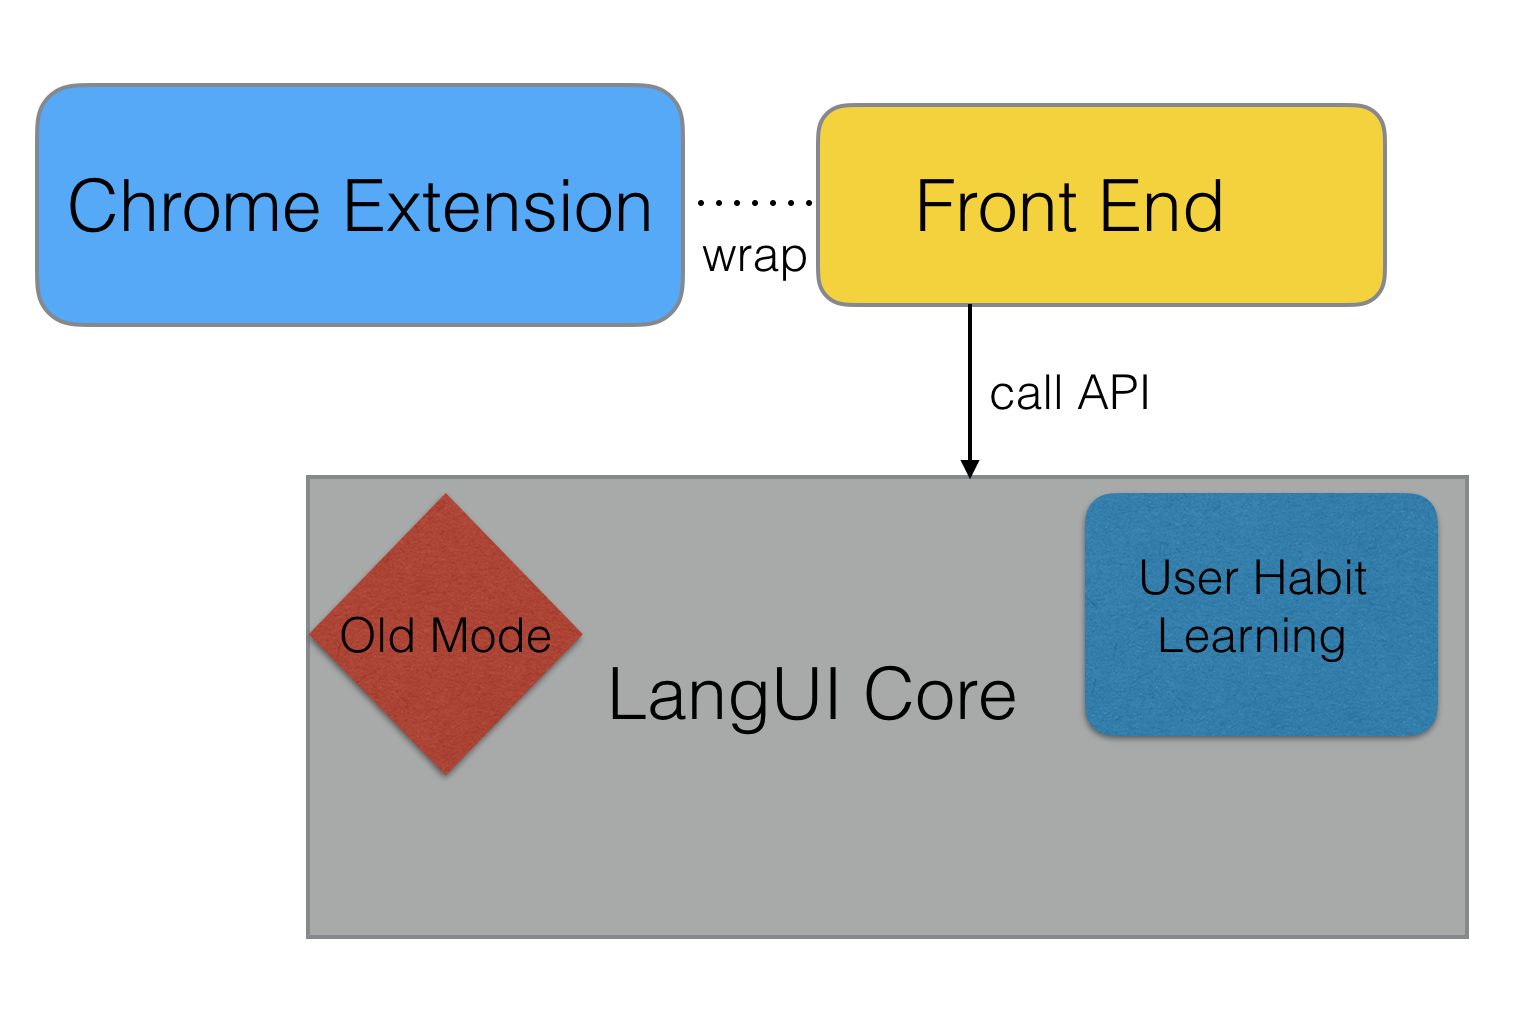
\includegraphics[width=8cm]{5.png}
\end{figure}

LangUI is composed of 3 parts: a Google Chrome extension wrapper, a html5 front end and LangUI core.

When you write some reports or paper, you are probably using a keyboard and a mouse. So I wouldn't consider tablets even though they are better devices for hand drawing. To make this tool more available,  cross-platform and lightweight, I decide to wrap it as Google Chrome Extension. The front end could be most likely written in html5. But it could change during implementation phase.

The LangUI core should provide the following features:

\begin{enumerate}
  \item Understanding users' strokes: Since users draws in LangUI's front-end, the speed and direction of strokes can be tracked. LangUI can analyze these features to guess the users' intension. For example, I would prefer to draw a "C" or "6" very quickly to embody the concept of "circle", LangUI should differentiate these strokes from a slow and smooth "C"/"6"-like curve.
  \item Tidying up the sketches to make them look like computer generated illustrations: LangUI should automatically generate smooth curves and straight lines. Automatic aligning is an optional feature.
  \item Old mode: It is the selecting and dragging mode. It is optional, but I do want to finish it as it could be a crucial supplement for the proposed workflow.
  \item Supervised learning: The LangUI learning submodule should track and learn users' preference on how to draw certain elements. The data coud be stored on a server and linked to their social media account. But I think simply using cookie is also acceptable in this scenario.  This feature is optional. If I don't have enough time, the default setting would be my personal preference.
\end{enumerate}

\subsection{Challenges}
It's really hard to beat state-of-the-art diagramming tools in usability. To achieve this goal, I have to make sure LangUI's understanding of users' intension is extremely accurate. Any misunderstanding would probably ruin user experience. Therefore the major challenge is how to optimize the stroke understanding module.

\section{Plan of Action}

\begin{enumerate}
  \item Feb 19 - March 4: Requirement engineering, system design,  enabling technology survey, front-end development.
  \item March 5 - March 18: 70\% Implementation of the LangUI core.
  \item March 19 - April 1: Implementation of the LangUI core and the front-end.
  \item April 2 - April 15: Implementation of optional features, evaluation and documentation.
\end{enumerate}





\section{Bibliography}

\begin{thebibliography}{1}

\bibitem{cmpsim}
 S.W.Draper, \emph{Practical Methods for Measuring Human-Computer Interaction}, Nov 2002. Link: http://www.psy.gla.ac.uk/~steve/resources/uipm.pdf.

\bibitem{mp}
John D. Hobby, \emph{Metapost: A User's Mannual}, May 21, 2014. Link: https://www.tug.org/docs/metapost/mpman.pdf.

\bibitem{ut}
T. Morales de Luna, \emph{Useful Vector Graphic Tools for LATEX Users}, in The PracTEX Journal, 2010, No. 1. Link: https://tug.org/pracjourn/2010-1/morales/morales.pdf.

\end{thebibliography}

\end{document}
